
\section{Task 2: Circuit Techniques to Improve Reliability, Yield and Density}
The advent of novel materials and devices have created many opportunities in circuit design. On one hand, the general requirements to all the memories are similar, i.e. high density, fast speed, low power, affordable yield and reliability, etc. On the other hand, each NVM technology faces different process integration difficulties, owns unique device characteristic, and targets on different memory market. Therefore, the primary concerns and the optimal solutions for different NVM chip designs are different. Our proposal is to investigate the common design issues and to exploit distinctive circuit techniques for each individual emerging NVM technology. More specifically, we will focus on three main concerns in emerging NVM design -- reliability, yield, and density.

\subsection{Task 2.1: Reliability Improvement}
Reliability is an important parameter in NVMs, which is usually evaluated by data retention and write endurance. While data retention is not a big issue for emerging NVMs (see Figure~\ref{table}), write endurance becomes one of the biggest obstacles that prevent them from massive production and commercialization. Write endurance is usually measured by the number of writes performed before the cell cannot be programmed reliably. SRAM and DRAM both have endurance of about $10^{16}$ programming cycles~\cite{ITRS07}, which are sufficient for use even in high-performance processors.

For different emerging NVMs, the physical mechanisms to cause endurance issues are different. In PCRAM, writing is a primary wear mechanism: when injecting current into phase change material, thermal expansion and contraction degrades the electrode-storage contact. Based on a survey of circuit prototypes published within the past five years, the best reported write endurance for PCRAM is 10$^9$~\cite{Lee09}. Currently, the best test result of STT-RAM write endurance is $\sim4\times10^{12}$ programming cycles~\cite{Diao07}. Theoretically MRAM should be able to be programmed $>10^{15}$ times~\cite{ITRS07} since its magnetic stack is similar to the one used in hard disk drive. The gap mainly comes from the immature process integration. In parallel to improving material and process development, circuit design techniques can help out in many ways.

\paragraph{Self-contained local control scheme.} In general, the damage on NVM material has an \textbf{\emph{exponential}} relationship with the current/energy applied on it. And it is an accumulative procedure of total time period. Hence, the most effective approach to improve write endurance is to reduce the write current ($I_{wr}$) and write operation period ($t_{wr}$).

For example, one possible solution is smoothing $I_{wr}$ shape during write operations and avoiding overshot on NVM materials. Accordingly, how to design a write driver to provide a sleek but fast ramp-up curve is tricky. Another interesting alternative could be lowering the voltage on memory device to meet only the minimal required current. Obviously, an accurate self-timing control scheme is necessary, which can stop providing writing current to memory cells once detecting successful programming operations. On one hand, we observe that a longer $t_{wr}$ is needed when a smaller $I_{wr}$ is provided. $t_{wr}$ could be very sensitive to $I_{wr}$, e.g. $t_{wr}\propto{-I_{wr}}$ in MRAM. On the other hand, the process variations at nano-scale technology node, including variations of both CMOS devices and NVM elements, make it very hard to control $I_{wr}$ precisely.

Hence, we propose to add a self-contained local control scheme. The scheme is \emph{\textbf{self-contained}} because it is mainly composed of a number of memory cells by using the same emerging NVM device. These cells are divided into three functional groups used for configuration, detection and control, respectively. The initial configuration should be programmed at testing stage before chip is shipped out. During write operations, the detection cells are also programmed and the degradation degrees of these cells can be used to predict the status of memory cells in the main array. The prediction result will be fed into control schemes periodically to adjust $I_{wr}$ and $t_{wr}$ on the fly. When needed, the control signals can even be used at system level, for example, to adjust the bit-redundancy or to select ECC algorithm. The granularity of the self-contained local control scheme depends on each specific NVM technology and its targeted applications.

\paragraph{Circuit techniques to enable wear leveling.} Architectural level techniques have been proposed to mitigate the endurance problems in PCRAM, such as \textit{Read-before-Write} or \textit{White Cancellation}~\cite{Lee09,PRAM:IBM}. In this task, we plan to investigate circuit-level techniques to enable wear leveling for NVM memories. Specifically, we plan to study two wear leveling techniques: (1) \textit{Bit-line Shifting:} Usually, write-operations in applications demonstrate an extremely uneven distribution in a memory block. Consequently, a few hot memory cells are worn out much faster than other cells, making the entire memory block useless even though most of the cells are still functional. Based on such observation, we plan to design a bit-line shifter to spread out the writes over all memory cells in a memory block. In our design, each memory block has its own shift offset register (SOR) and shift interval counter (SIC). An SOR stores the shift offset of its cache block, and the bit-line shifter refers to it to determine how many bits to shift the incoming data before store it to the cache block. An SIC records the number of writes performed to its cache block, and when it reaches to a predefined threshold, we update the corresponding SOR value. Hence, we can achieve the balance between the wear-leveling performance and the additional bit changes caused by changing shift offsets. (2) \textit{Word-line Remapping:} Similar to Bit-line shifter, we can also use a word-line remapper to spread out writes over all cache blocks. The word-line remapper consists of an adder and a word-line SOR to keep the current word-line shift offset, through which a word-line decoder logic can determine what word-line should be enabled. After changing the value of the word-line SOR, we should invalidate the contents in the cache because the word-line mapping is changed. Therefore, the word-line remapping period should be long enough (e.g., a second) to avoid excessive remapping overhead. These two circuit-level modification to the memory array will be evaluated on the effectiveness of the endurance improvement, as well as the performance/area/energy overhead, and will be compared against architectural level techniques such as those proposed in~\cite{Lee09,PRAM:IBM}.

\paragraph{Multi-level cell (MLC) write endurance.} Multi-level cell (MLC) can effectively improve the integration density of memory by storing more than one bit information in a single memory device: $n$ bits are represented by  $2^n$ states of a storage device. The success of MLC in NAND flash memory has been explored in PCRAM~\cite{Raoux08,Bedeschi09}, STT-RAM~\cite{Lou08}, and RRAM~\cite{Baek05}. MLC can effectively improve the integration density of memory. However, the write endurance is degraded significantly due to the smaller resistance gap between two adjacent states. In the project, we will seek optimal solutions to improve MLC write endurance by considering write patterns of both physical mechanism and system requirement.

\begin{figure}
\centering
\vspace{-10pt}
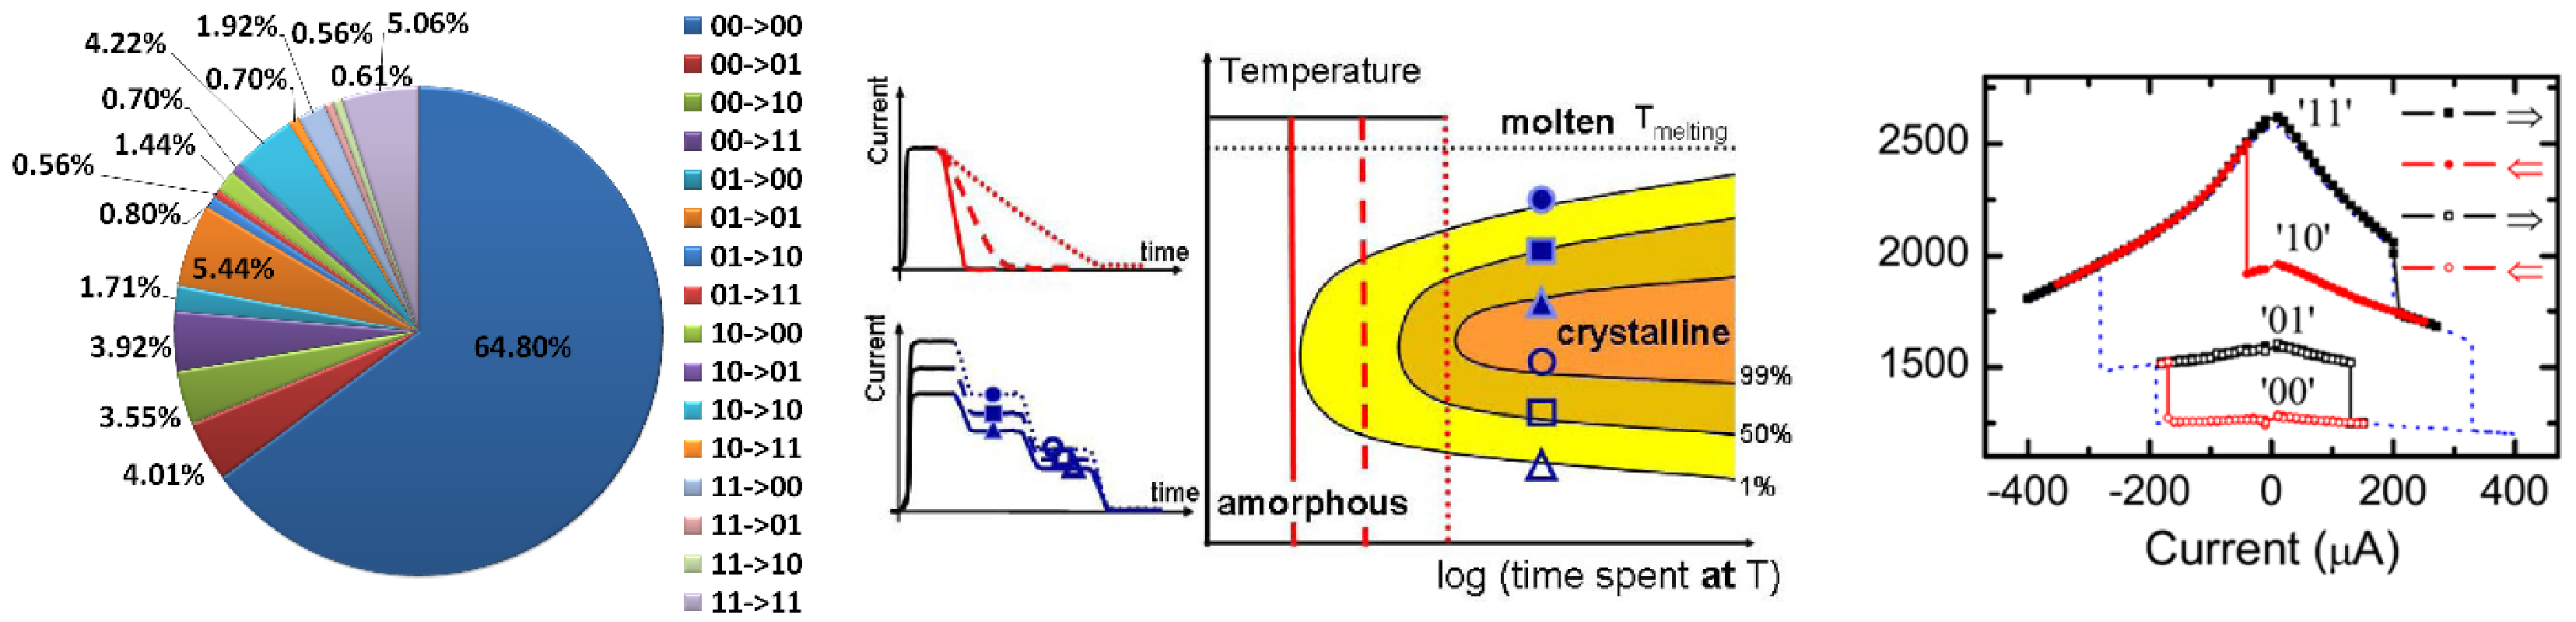
\includegraphics[width=1.0\textwidth]{./figure/4_mlc.pdf}
\vspace{-10pt}
\caption{MLC write patterns. \underline{Left:} The transition distribution between the different values of MLC MRAM bit; \underline{Middle:} PCRAM -- Schematic plot of time-temperature-transformation-chart~\cite{Nirschl07}; \underline{Right:} MRAM R-I sweep curve~\cite{Lou08}.}
\label{mlc}
\vspace{-10pt}
\end{figure}

Let's use a 2-bit MLC as an example. Each memory cell can represent four logic states, namely $L00$, $L01$, $L10$, and $L11$.  Figure~\ref{mlc} shows the transition distribution between the different logic values in an in-order microarchitecture. We noticed that most of transitions occur between the same values, and hence, there is no need to change resistance state at all. The observation is can be extended to most of embedded applications as well. Therefore, ``write-after-read'' scheme, which conducts only the necessary transitions based on the values of the new data being written and the original data stored in the MLC bit, could be the most efficient way for energy saving and lifetime improvement. However, the extra read in write operation results in performance overhead. How severe is the performance overhead? Can it be absorbed or minimized? Can we detect the data in memory cell at the same time as cell is programmed and terminate the writing earlier? These questions will be discussed in the project.

Assume the four resistance states of a 2-bit MLC are $R00$, $R01$, $R10$, and $R11$, from low to high. We noticed that switching to different resistance state in an MLC need follow specific sequence and/or demand different write current. As shown in Figure~\ref{mlc}, the multiple resistances in PCRAM are achieved by different size and shape of the amorphous region at the top of the pillar-heater within the phase change material. Hence, the target resistance strongly depends on temperature and time during write operations. An MRAM MLC requires a two-step writing, i.e. a large current switching followed by a low current one. This is because it has two free layers whose magnetization directions need to be switched separately. 

Corresponding to the four resistance states, an MLC cell has total of $4! = 24$ encoding schemes for its four logic states. As we stated above that the breakdown probability of a NVM cell has an exponential relationship with the current amplitude through it, the damage to memory material has different weight when writing different data. Properly selecting the encoding scheme of logic vs. physical states based on the transition distributions can further improve the write endurance and lifetime of MLC NVM technologies.

\subsection{Task 2.2: Yield Enhancement}
Higher defect rates and low yield are brought by the continuous shrinking of devices and the unlimited demand on higher densities. As technology enters into nanometer scale, device parameter fluctuations induced by process variations have become critical issues~\cite{Asenov03}. Emerging non-volatile memories, which are the densest circuits in systems, are greatly impacted by the large process variations. For example, MTJ resistance in MRAM increases exponentially with the thickness of oxide barrier between two magnetic layers. It was reported in~\cite{Tehrani00} that MTJ resistance increases by 8\% when the thickness of oxide barrier changes from 14${\AA}$ to 14.1${\AA}$. In the project, we propose to overcome the impact of process variations and to enhance yield by taking the advantage of the unique device characteristics of NVMs.


\begin{figure}
\centering
\vspace{-10pt}
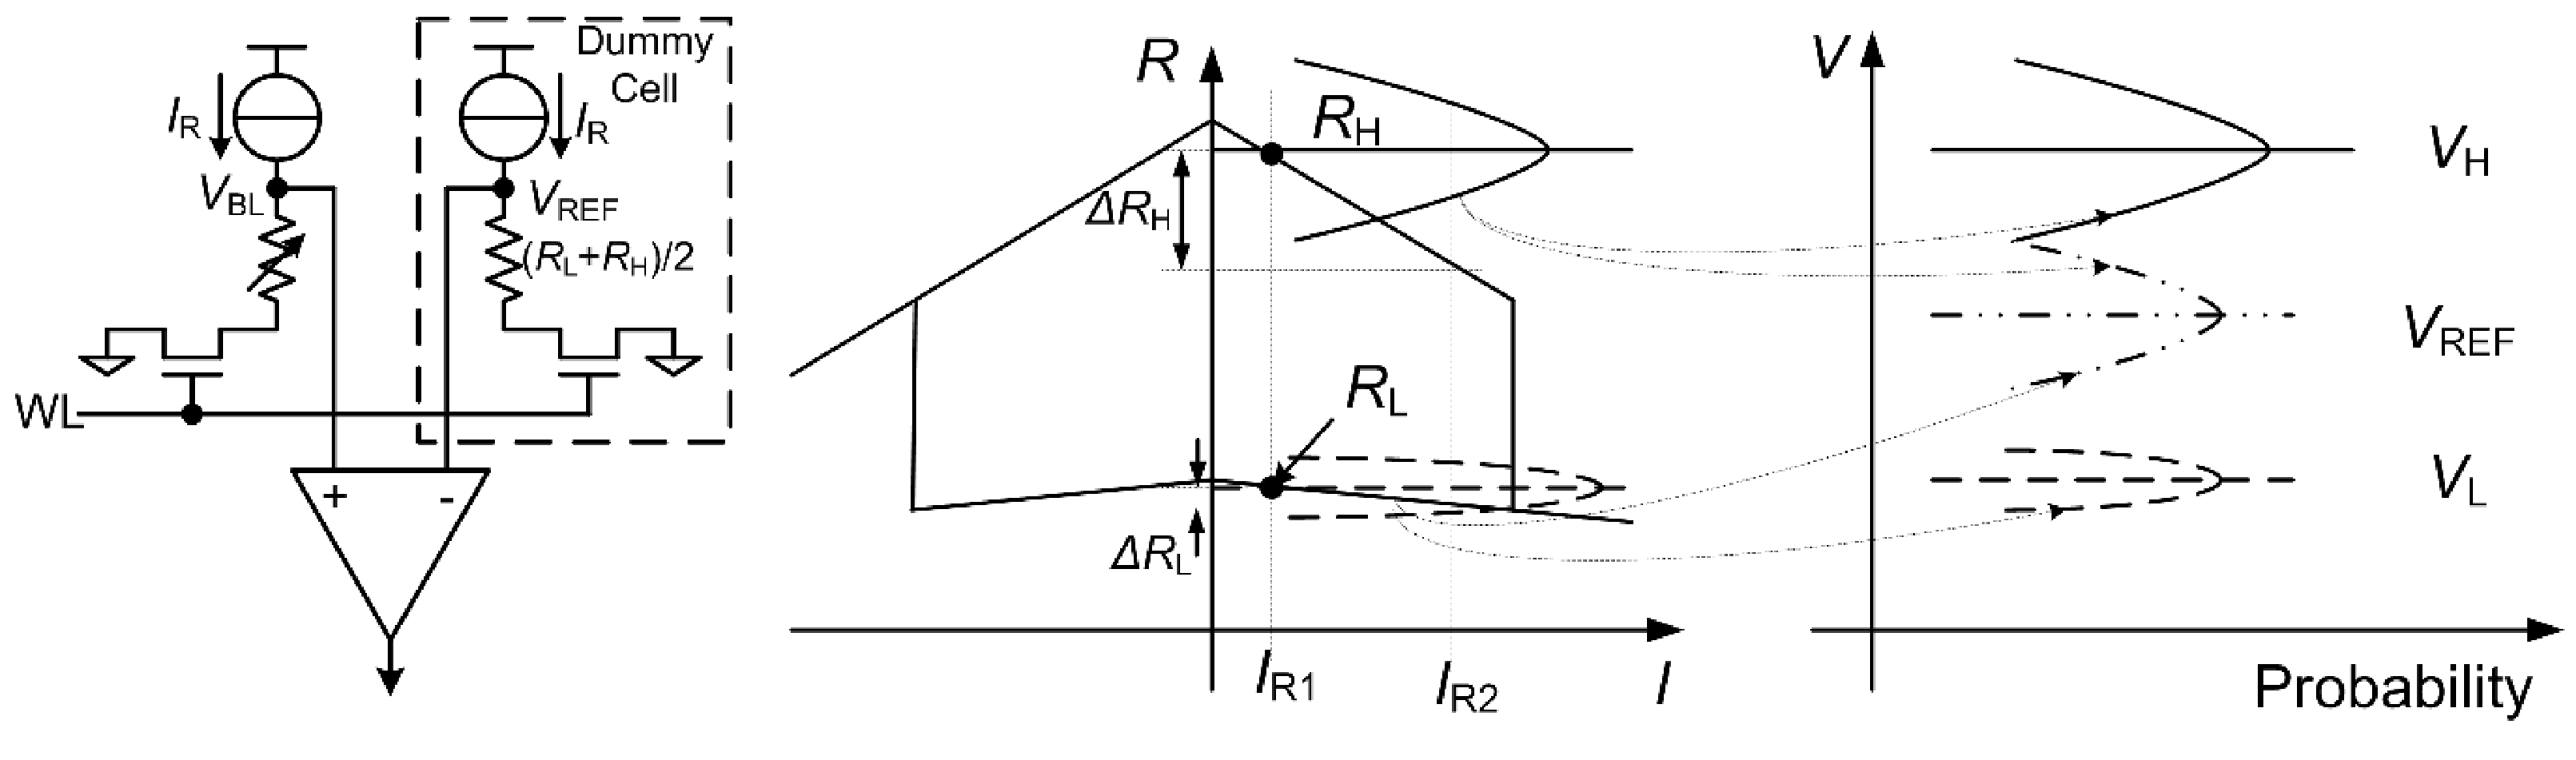
\includegraphics[width=0.85\textwidth]{./figure/5_selfref.pdf}
\vspace{-10pt}
\caption{\underline{Left:} Conventional read-out scheme of MRAM; \underline{Middle:} R-I characteristic of MgO-based MTJ; \underline{Right:} MTJ resistance distribution incurred read failure~\cite{Li09}.}
\label{selfref}
\vspace{-10pt}
\end{figure}

\paragraph{Non-destructive self-reference technology in MRAM.} Like most of the emerging NVM technologies, MRAM uses device resistance as the data storage media. Figure~\ref{selfref} shows a conventional voltage sensing scheme, which compares the bit line voltage $V_{BL}$ generated by the selected memory cell with a reference signal $V_{REF}$ produced by the dummy cell. A dummy cell is shared by multiple memory cells to reduce overhead. Ideally the resistance of the dummy cell should be set in the middle of the high and low resistance states ($R_H$ and $R_L$). In reality, process variation incurs the resistance distribution of MTJ in memory cells as well as the dummy cells. When the resistance variation $\sigma_R$ is large, the tails of $R_H$ or/and $R_L$ could be overlapped with $R_{dummy}$ and lead to the false detection of the stored value as illustrated in Figure~\ref{selfref}. We called it as \textbf{\emph{Read Failure}}.

Read failure is a severe problem in STT-RAM design for two main constraints: (1) The difference between two resistance states of MTJ is fairly small: $\Delta$R=$R_H-R_L$ $\approx$ $1000\Omega$ at 45nm technology node~\cite{Li09}; and (2) the MTJ resistance variation $\sigma_R$ is relatively high because it is extremely difficult to control oxide barrier thickness within a small range of variation, i.e. $0.5{\AA}$~\cite{Jeong03}. Besides the regular yield improvement techniques, such as redundant column/row and ECC, a self-reference read-out scheme could be another effective way to fix read-failure problem.

The basic idea of a self-reference reading is to compare the stored data in a memory cell with a reference value written to the same cell. By limiting the comparison within one single STT-RAM cell, the impact of bit-to-bit variation of MTJ resistance can be avoided. Previously some self-reference schemes were used in toggle-mode MRAM design~\cite{MRAM:TTO+06,Jeong03}. We also successfully utilized it in STT-RAM design~\cite{Li:147723}. These schemes are all ``destructive'' because the original value in memory cell is wiped out when writing the reference value into MTJ, and has to be recovered at the end of the read operation. Obviously it prolongs read latency and aggravate reliability issue.

In this project, we will work on a \textbf{\textit{non-destructive self-reference}} methodology, which does not disturb the original data during read operations. The approach comes from the special R-I characteristic of MgO-based MTJ. As we can see in Figure~\ref{selfref}, the MTJ current dependence of $R_H$ and $R_L$ are quite different: the current roll-off slope of $R_H$ is much steeper than that of $R_L$. Therefore, we can sample the stored value of an MTJ twice by using two read currents $I_{R1}$ and $I_{R2}$ and compare the resistance difference ${\Delta}R=R1-R2$. Obviously ${\Delta}R_H$ is pretty big, while ${\Delta}R_L$ is close to `0'.

To approve the feasibility of this approach, more details on circuit design need to be analyzed. For example, how much is the sensing margin in the new read-out scheme after considering process variations? Is it tolerable within current sensing scheme? Will a new sense-amplifier (SA) design be necessary? How does it impact memory array structure? How much yield improvement can be achieved with the new scheme? Will this scheme be still valid when technology further scales down? In this proposal, we will investigate these issues and exploring the solutions. Our target is minimizing the impacts of process variations at the same time improving read performance.

\paragraph{Resistance drift.} Resistance drift has been observed in both PCRAM and memristor-based memory. In PCRAM, especially multi-level memory, the amorphous phase (and other phases obtained by incomplete phase transition) is metastable and can experience structural relaxation~\cite{Pirovano04}, which results in resistance drift over the time. For a memristor-based memory, if the read operation cannot provide zero flux, the resistance could ``drift'' to one direction continuously due to the accumulative effect of the input flux~\cite{Ho09}. Resistance drift can increase resistance variation $\sigma_R$ and hence, spread out the resistance distribution. Memory access patterns (e.g. the resistance state stored in the cell, read/write access frequency and interval, etc) strongly impact the resistance drift. On top of the process variations, the resistance drifts make the design margin even smaller, which aggravates read failure and further hurt chip yield.

The resistance drift in memristor-based memory design is mainly impacted by read access frequency. Ho et. al. proposed a refreshing scheme: after a particular number of reading operation, a refresh operation is needed to eliminate the effect of read pulse mismatch~\cite{Ho09}. We propose to flip the read current direction whenever accessing the memristor. The difficult part of this approach is to determine the granularity. Obviously a fine granularity is more effective to overcome the resistance drift in memristor. However, it also results in high performance and area overhead to record/achieve all the required information, i.e. previous read current directions. On the contrary, a coarse granularity could reduce the overhead, but it may not help much in the worst situation.

The resistance drift in multi-level PCRAM has a different behavior pattern from memristor-based memory. It is determined only by the state stored in the cell and interval to the previous write, no matter if the chip is powered up or accessed. Xu and Zhang~\cite{Xu10} proposed to solve the resistance drift in PCRAM with a complex ECC, which can minimize the error rate to a sufficient low level during its whole lifetime. The drawback of the scheme is the large overhead on performance and circuit complexity. Instead, we propose to build a self-adjustable sensing scheme, in which the reference current/voltage can be self-adjusted to follow the trend of resistance drift. Phase change material or memristor-based material could be used to monitor the device degradation. Similar to our proposal for memristor-based memory, properly selecting granularity and covering the worst-case situation will be the key issues to be investigated in the project.

\subsection{Task 2.3: High Density}
Increasing memory density is an ultimate goal in memory design. In the past, technology scaling is always the biggest driving force to reduce single cell size. Process development plays an important role as well. For example, to continue scalability, the charge storage materials of NAND Flash have gone through several generations: from standard double polysilicon gate, to SONOS, to bandgap engineered SONOS, and to TaNOS~\cite{Lu09}. Circuit design techniques play an important role to boost memory density too. For example, word-line overdrive scheme used to reduce select transistor size in memory cell~\cite{Li09}. In the project, we propose to introduce novel devices into emerging NVM design for density enhancement and investigate the corresponding design techniques.

\paragraph{Double cell configuration in bipolar switching RRAM.}
In RRAM design, crossbar structure is widely investigated. In each cell, only two terminals are needed -- one is horizonal (WL) and another is vertical (BL). The storage element is built at the cross-point of two metal wires. A diode could be used as selective element in unipolar switching RRAM. When RRAM material is bipolar switching, a non-ohmic device (NOD)~\cite{Yan4430255} is needed to provide two-direction driving current and to support process integration of cross-point structure. We call it as 1NOD-1R as shown in Figure~\ref{doublecell}. Data access is supported by properly controlling the voltages applied on WL's and BL's. Theoretically, crossbar structure has the smallest memory cell area 4$F^2$. Here, $F$ represents the technology feature size.

Due to process limitation, 1NOD-1R cell structures are facing some design difficulties. Conceptually, NOD can be understood as two parallel connected diodes. Ideally, it turns on only when the voltage drop between the two terminals exceeds its threshold. However, the I-V characteristic curve of real device could be quite different. This results in sneak path which has three or more cells in series as shown in Figure~\ref{doublecell}. The sneak current can introduce disturbance on unintended cells during read, write and erase operations.

Here, we propose to build a double cell configuration in bipolar switching RRAM by stacking two cells back to back with a barrier layer in between. Figure~\ref{doublecell} illustrates such a double cell by using PMC material as example: The PMC with active electrode on top is used as data storage (RRAM), while the main function of the PMC with active electrode at bottom is the selective device. The functionality of the proposed structure is guaranteed by the asymmetric I-V characteristic of PMC -- a higher voltage is required in RESET operation ($V_r$) than the one in SET operation ($V_s$). A large $I_{on}$/$I_{off}$ ratio (large turn-on current $I_{on}$ and extremely small turn-off current $I_{off}$) due to the big different between the high and low resistance states minimizes the disturbance from sneak current.

The integration of the proposed structure is friendly to CMOS technology since RRAM technology itself is compatible to CMOS process. However, to make this structure feasible to production, there are still many device and design details to be discussed. For example, to guarantee the correct functionality, the timing sequence need be adjusted. Consequently, the peripheral circuit design and floorplan need to be re-designed. The impacts of process variations need to be considered too. Furthermore, what kind of device characteristic is favorable in such a structure? Will we be able to expand this structure to other RRAM and memristor-based memory design? In this project, we will address these issues and explore solutions.

\begin{figure}
\centering
\vspace{-10pt}
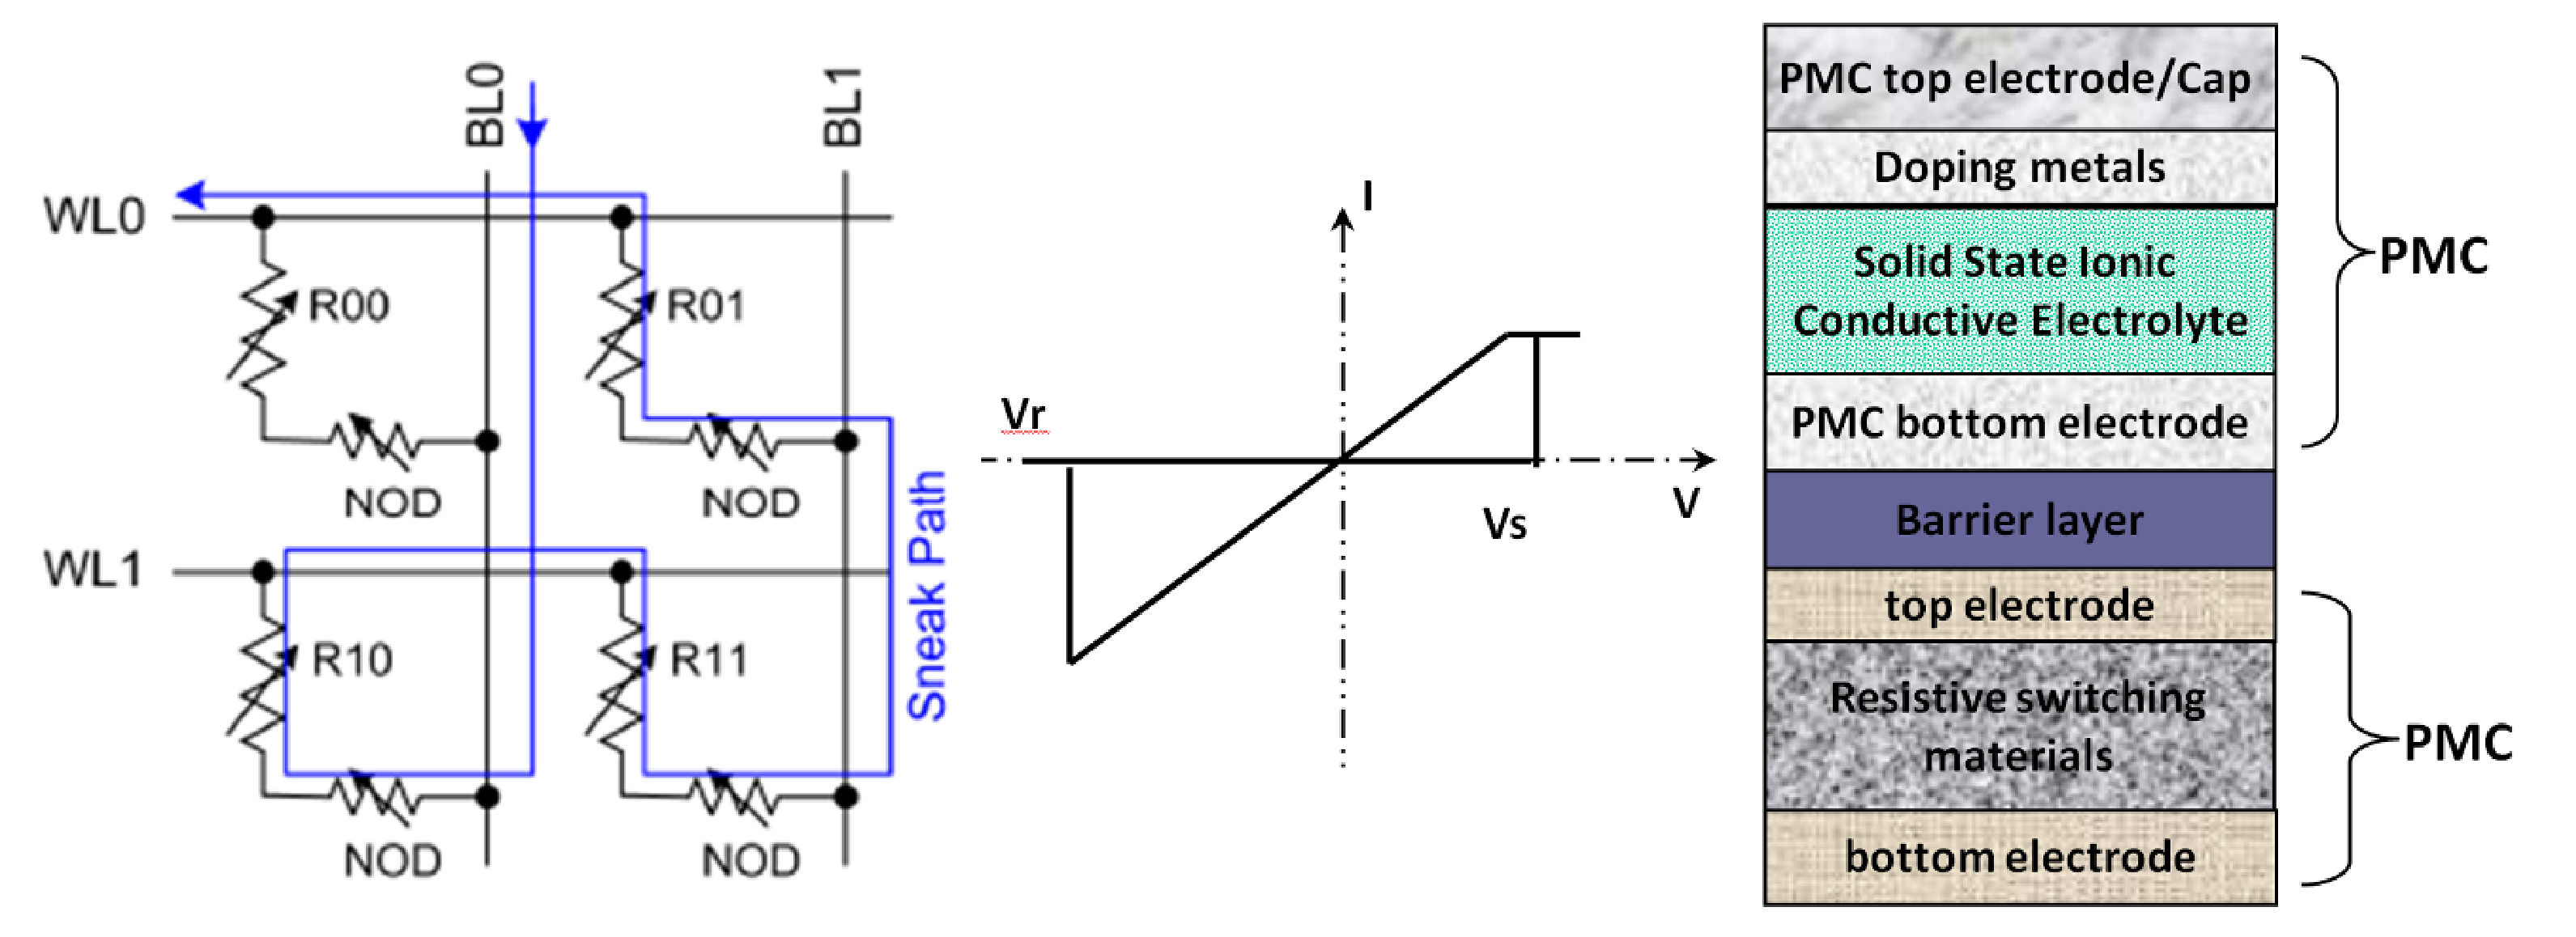
\includegraphics[width=0.75 \textwidth]{./figure/6_doublecell.pdf}
\vspace{-10pt}
\caption{\underline{Left:} 1NOD-1R and sneak path; \underline{Middle:} R-I characteristic of PMC; \underline{Right:} double cell configuration by stacking two cell back to back with a barrier layer in between.}
\label{doublecell}
\vspace{-10pt}
\end{figure}

\paragraph{3-D stacking peripheral circuitry.}
RRAM crossbar structure can also grow in third dimension, which is called intra-die stacking. The memory storage cell is located in between any two adjacent metal layers which are used as interconnects. Within the same die size, the multiple memory layers further improve memory capacity. If we still use the bottom layer as logic layer and connect upper memory layers through via holes, the area of  peripheral circuit will increase significantly, and hence cut down the high-density effect introduced by the intra-die stacking structure. Therefore, a 3-D stacking peripheral circuitry become necessary in order to increase array efficacy.

Previously, Song et. al. showed GIZO thin film transistors (TFTs) can be stacked vertically and might be used in intra-die memory~\cite{Song08}. However, their work still remained at material level. In this project, we will further explore it in device and circuit design level. The initial proposal in ~\cite{Song08} was to use TFTs as word-line (WL) selection transistor only. It does not reduce the number of via holes from bottom layer to upper memory layers because WL's has the identical number as the inputs of WL drivers. We plan to explore the usage of TFTs to some simple logic functions, e.g. the last stage of WL decoder. In such a case, only signals from pre-decoding schemes need to be fed into each memory layer. Hence, the functional blocks on the logic layer and the via holes connecting different layers can be dramatically reduced.

Design of such a hybrid circuit will be very challenging but interesting because new device can bring more constraints, which again motivate the invention of new design techniques. Also, many details need be discussed in the approach. For example, how to arrange TFT layout to fit into the small pitch of crossbar array? And how to build power supply network in 3-D stacking peripheral structure? Depending on the process development status, we even can exploit it to more complex functional blocks and further improve the density of peripheral circuitry. Besides TFT, we will keep an eye on any other emerging devices with the potential for 3-D stacking logic design.

\subsection{Preliminary Results and Collaborations:}
The NYU-Poly PI Li has worked on memory design for years, from traditional SRAM to current emerging NVMs. Her research on low-power SRAM design ~\cite{Agarwal02,Agarwal03,Bhunia02} has been used in Intel processor. In Seagate, she has led a design team on MRAM and RRAM test-chip design and proposed many circuit techniques to improve reliability~\cite{Chen:198516,Li:502194}, yield~\cite{Li:147723,Chen:147727} and density~\cite{Li:242331,Chen:170549,Li:250027,Li:426098} of emerging NVMs. The PSU PI Xie has rich experience in SRAM-based cache design~\cite{Xie:TC09,XIE:TVLSI2008-3DCacti,Xie:MTDT09,Xie:ISCA09,xie:iccd05-3d}, PCRAM-based cache design~\cite{xie:glsvisl08-pram}, and MRAM-based cache design~\cite{XIE:HPCA09,Xie:dac08} (in collaboration with the NYU-Poly PI Li) .

